\documentclass[12pt]{article}
\usepackage[margin=1in]{geometry}     
\usepackage{graphicx}
\usepackage{epstopdf}
\setlength\parindent{0pt}
\usepackage{natbib}
\usepackage{booktabs}
\bibliographystyle{plainnat}
\usepackage{soul}
\usepackage{subcaption}
\usepackage{booktabs}
\usepackage{array}
\usepackage{threeparttable}
\usepackage{rotating}
\usepackage{pdflscape}
\usepackage[fleqn]{amsmath}

\usepackage[format=plain,
labelfont=it,
textfont=it]{caption}

\newcommand{\FCO}{F$_{\mathrm{CO}_{2}}$}
\newcommand{\CO}{CO$_{2}$}

%opening
\title{Quantifying Historical F$_{\mathrm{CO}_{2}}$ Timeseries}
\author{Riley X. Brady}
\date{\today}


\begin{document}

\maketitle
\begin{abstract}
\noindent Thus far, the study has focused on understanding the residuals of \FCO, by removing the CESM-LENS ensemble mean from each individual simulation. It has been assumed that these residuals exactly represent the natural flux of carbon. However, embedded in the ensemble mean is a seasonal cycle that might very well contain some of the natural \CO~fluxes. I am backtracking in this phase of the project to be confident in our definition of these residuals. In the process, I will also quantify various aspects of the historical `mean state' of each system.
\end{abstract}

\section{What exactly are our residuals and seasonal cycle representing?}
It isn't immediately clear what our ensemble mean and residuals represent in the case of \FCO over the historical period in the CESM-LENS. We can assume that the ensemble mean trend represents the growing anthropogenic \CO~sink in the ocean, but what about the seasonal cycle? Surely the seasonal cycle cannot be purely due to anthropogenic forcing, but rather it is the seasonal cycle that all members share in common. How much of that seasonal cycle is anthropogenic versus natural, and what controls it? \\

Figure~\ref{fig:calcs-timeseries} displays the issue with understanding what each component of the time series represents. We can assume that any trend in the forced signal (red line) is due to the invasion of anthropogenic carbon. However, the seasonal cycle (the black curve) must at least partially represent natural carbon. So are the grey lines (residuals) just truthfully the natural variability of \CO? Do these residuals include any anthropogenic carbon? \\
\clearpage
\begin{figure}[!h]
	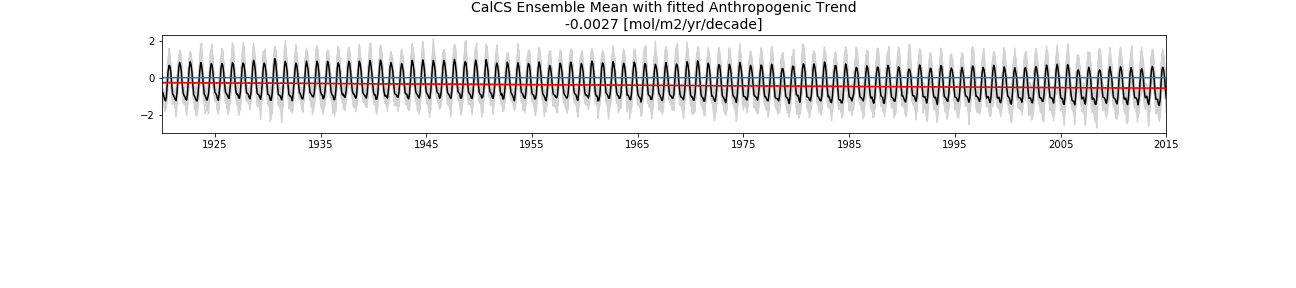
\includegraphics[width=\linewidth]{figs/CalCS_timeseries.png}
	\caption{Historical time series of \FCO in the California Current across the CESM-LENS. The black line represents the ensemble mean, the red line a linear trend, and the grey the residuals.}
	\label{fig:calcs-timeseries}
\end{figure}

We can explore this question by using the FG\_ALT\_CO2 output from the CESM-LENS. This output represents the \CO~flux when run from 1920-2100 with pre-industrial emissions. Thus, there is no anthropogenic carbon involved in this simulation. The difference between \FCO and FG\_ALT\_CO2 is then anthropogenic carbon. (See \citep{lovenduski_enhanced_2007} for more details)



\clearpage
%\begin{figure}[!h]
%	\centering
%	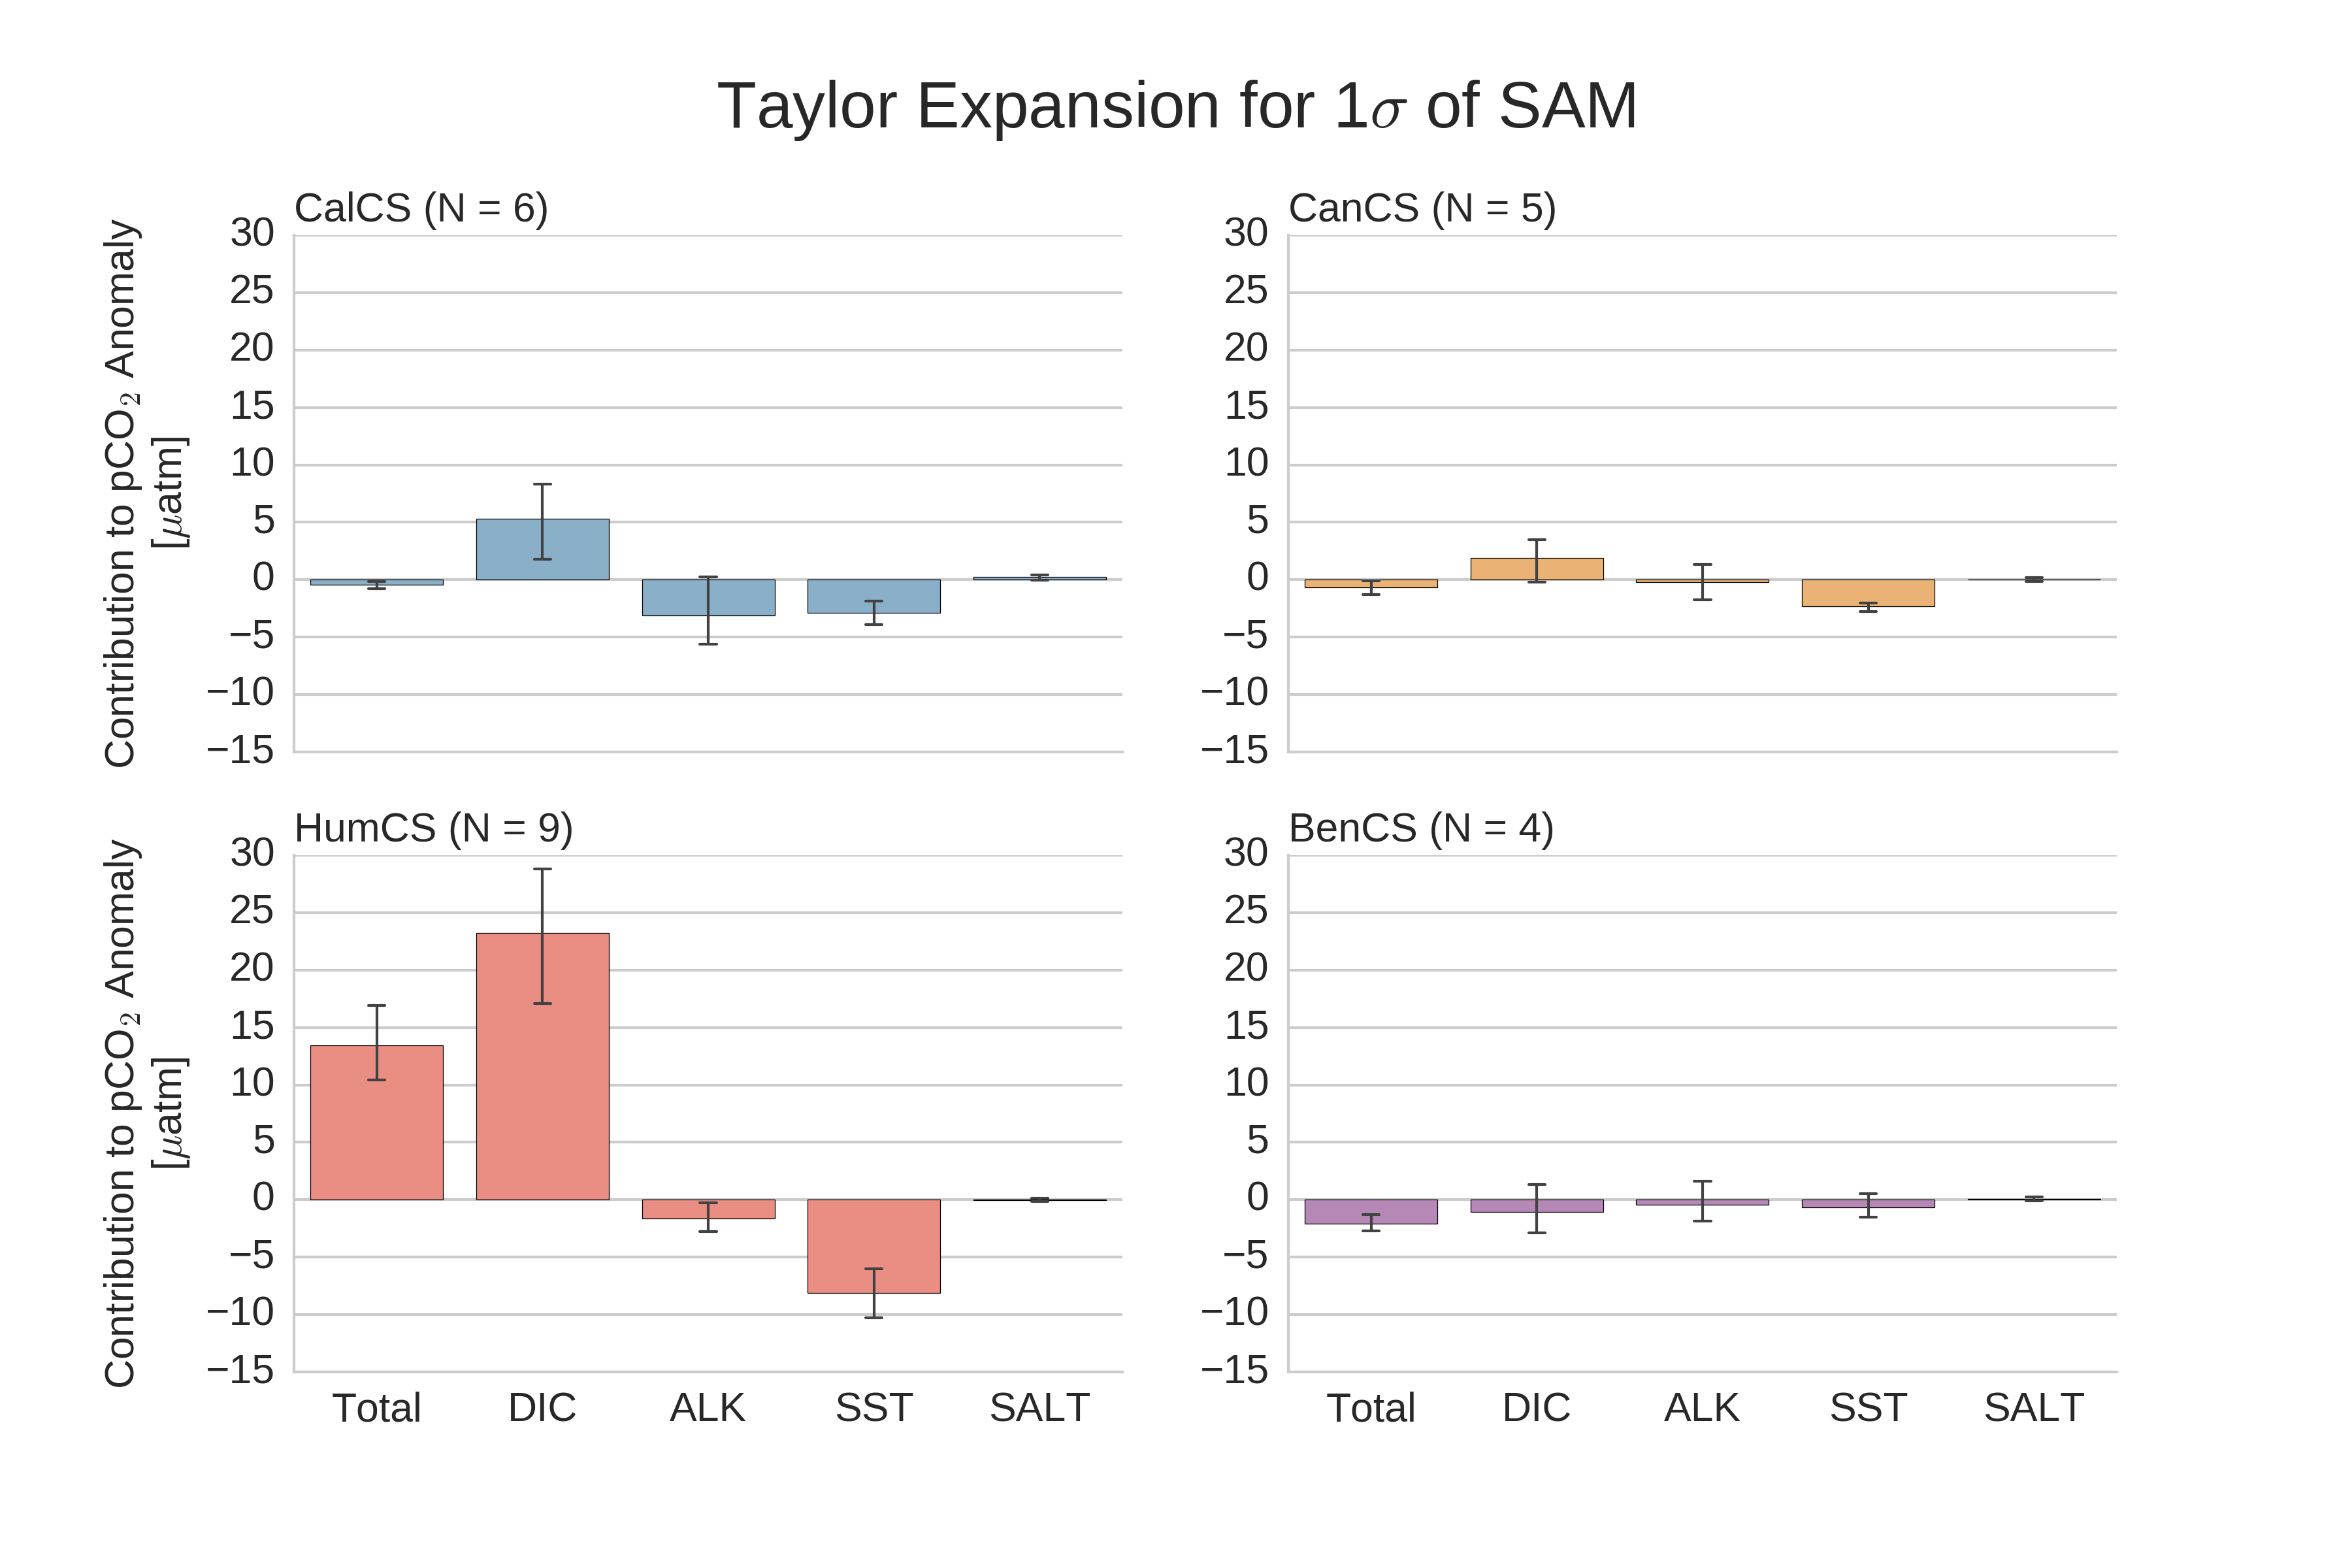
\includegraphics[width=\linewidth]{../../figs/all-systems/taylor_expansions/taylor-expansion-SAM-pCO2-PVALUEREMOVED-smoothedClimate.png}
%	\caption{Linear Taylor Expansion of the relative contributions toward pCO$_{2}$ anomalies in a 1 $\sigma$ SAM event. Only simulations with $p$ $<$ 0.05 for pCO2, SALT, SST, ALK, and DIC were included.}
%	\label{fig:taylor-sam}
%\end{figure}

\clearpage
\bibliography{../../EBUS_BGC_Bibliography.bib}
\end{document}